% @Author: AnthonyKenny98
% @Date:   2020-04-08 15:17:43
% @Last Modified by:   AnthonyKenny98
% @Last Modified time: 2020-04-08 16:02:17
\begin{figure}
\begin{centering}
\begin{tabular}{c}

\begin{subfigure}{0.97\linewidth}
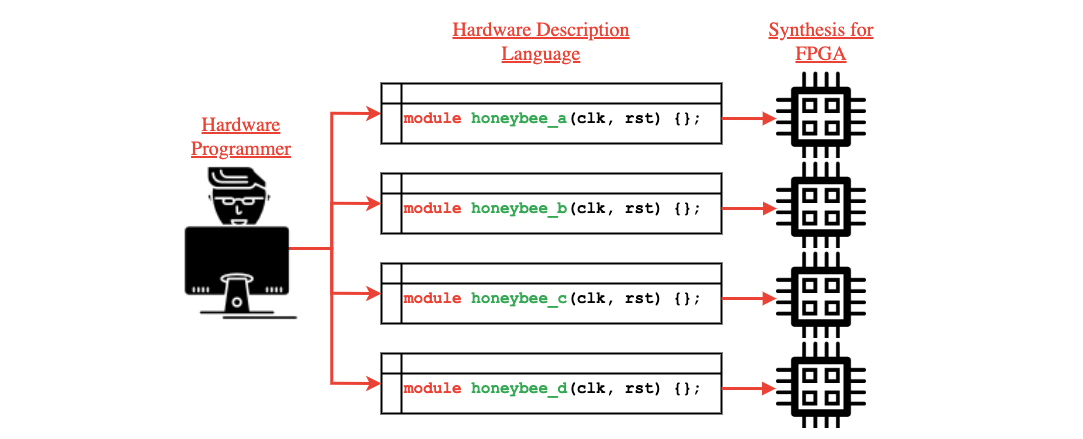
\includegraphics[width=\linewidth]{chapters/chapter3/img/hls_to_fpga_a.png}
\caption{Hardware Optimization without HLS}
\label{fig:hls_to_fpga_a}
\end{subfigure} \\

\begin{subfigure}{0.97\linewidth}
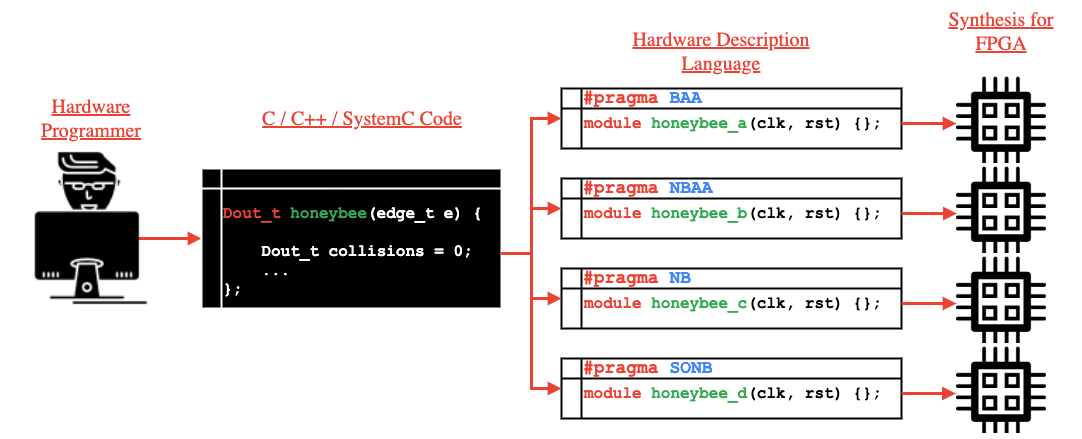
\includegraphics[width=\linewidth]{chapters/chapter3/img/hls_to_fpga_b.png}
\caption{Hardware Optimization with HLS}
\label{fig:hls_to_fpga_b}
\end{subfigure}

\end{tabular}
\mycaption{Hardware Optimization Process}{. Figure \ref{fig:hls_to_fpga_a} shows how, without using HLS, the hardware developer must write multiple different implementation of the same functionality to acheive different performance. Figure \ref{fig:hls_to_fpga_b} shows how, when using HLS, the hardware developer only must write one implementation (in a higher-level language like C), and then use ``pragmas'' to create different implementations (with different optimizations) for synthesis.}
\label{fig:hls_to_fpga}
\end{centering}
\end{figure}